\documentclass[conference]{IEEEtran}
\IEEEoverridecommandlockouts

\usepackage{cite}
\usepackage{amsmath,amssymb,amsfonts}
\usepackage{booktabs}
\usepackage{array}
\usepackage{graphicx}
\usepackage[hidelinks]{hyperref}

\newcolumntype{L}[1]{>{\raggedright\arraybackslash}p{#1}}
\newcolumntype{C}[1]{>{\centering\arraybackslash}p{#1}}

% --- Draft placeholders -------------------------------------------------
% \TBD marks a cell or value reserved for a MEASURED quantity. It is not an
% estimate, a prediction, or an expected result. Replace every occurrence
% with a logged number before submission; search the source for "TBD".
\newcommand{\TBD}{\textsc{tbd}}
% \figbox renders a visible, compiling placeholder for a figure that has not
% been produced yet. Replace the whole call with \includegraphics.
\newcommand{\figbox}[3]{%
  \fbox{\begin{minipage}[c][#2][c]{#1}\centering
  \scriptsize\textsc{figure placeholder}\\[3pt]#3
  \end{minipage}}}
% ------------------------------------------------------------------------
\setlength{\textfloatsep}{7pt plus 1pt minus 2pt}
\setlength{\floatsep}{6pt plus 1pt minus 2pt}
\setlength{\intextsep}{6pt plus 1pt minus 2pt}

\title{DenseNet--Swin Transformer Classification with Evidence-Constrained Summarization of Pneumonia Radiography}

\author{
\setlength{\tabcolsep}{3pt}%
\begin{tabular}{ccc}
\begin{tabular}{c}
1\textsuperscript{st} \textit{Tejonidhi M R}\\
\textit{Malnad College of Engineering,}\\
\textit{Karnataka, India}\\
tmr@mcehassan.ac.in
\end{tabular}
&
\begin{tabular}{c}
2\textsuperscript{nd} \textit{Nandan H S}\\
\textit{Malnad College of Engineering,}\\
\textit{Karnataka, India}\\
nandanhs.146@gmail.com
\end{tabular}
&
\begin{tabular}{c}
3\textsuperscript{rd} \textit{Poorab N G}\\
\textit{Malnad College of Engineering,}\\
\textit{Karnataka, India}\\
poorabng@gmail.com
\end{tabular}
\\[1.1em]
\multicolumn{3}{c}{
\begin{tabular}{cc}
\begin{tabular}{c}
4\textsuperscript{th} \textit{Kushal H S}\\
\textit{Malnad College of Engineering,}\\
\textit{Karnataka, India}\\
kushalhs456@gmail.com
\end{tabular}
& \hspace{4em}
\begin{tabular}{c}
5\textsuperscript{th} \textit{Poornachandra N}\\
\textit{Malnad College of Engineering,}\\
\textit{Karnataka, India}\\
poornagowda425@gmail.com
\end{tabular}
\end{tabular}
}
\end{tabular}
}

\begin{document}
\bstctlcite{IEEEexample:BSTcontrol}
\maketitle

\begin{abstract}
Chest radiographs are routinely used to assess pneumonia, but a classification probability alone does not show how a model reached its decision. This paper presents an image-analysis pipeline that combines DenseNet121 and Swin Transformer-Tiny (Swin-T) for binary classification of pediatric chest X-rays as normal or pneumonia. DenseNet121 captures local radiographic patterns, while Swin-T models wider spatial relationships. Their feature maps are aligned, projected, concatenated, and refined with a post-fusion Convolutional Block Attention Module (CBAM) before classification. Grad-CAM provides a gradient-based heatmap from the fused representation, and LIME supplies a complementary perturbation-based explanation. A deterministic serializer converts the probability and explanation outputs into neutral evidence fields. Gemini 3.5 Flash-Lite receives only this structured evidence and returns a short JSON summary under a fixed schema. Validation rules, a bounded correction attempt, and a deterministic template fallback block summaries that violate the permitted schema or recorded evidence. The system is implemented in PyTorch behind a service interface that exposes classification, explanation, and summarization as separate endpoints, and uses the public Kaggle Chest X-Ray Images (Pneumonia) dataset. Classification, explanation, and language generation remain separate, allowing displayed statements to be checked against recorded model outputs. The system is intended for technical research and education, not clinical diagnosis.
\end{abstract}

\begin{IEEEkeywords}
chest radiography, pneumonia classification, DenseNet121, Swin Transformer, CBAM, Grad-CAM, LIME, explainable artificial intelligence, constrained summarization
\end{IEEEkeywords}

\section{Introduction}
Pneumonia remains an important cause of childhood mortality worldwide \cite{who2026childmortality}. Chest radiography supports its assessment, though reading a film is affected by acquisition quality, projection, overlapping anatomy, and variation between observers \cite{lim2021pneumonia}. Deep networks pick up useful patterns in these images. What they do not supply is any account of which regions produced a given score.

Convolutional neural networks (CNNs), particularly DenseNet \cite{huang2017densenet}, are effective at encoding local texture and morphology. Hierarchical vision transformers such as Swin Transformer \cite{liu2021swin} complement this behavior by modeling longer-range spatial relationships through shifted-window attention. The system combines both representations and uses CBAM \cite{woo2018cbam} to refine the fused feature tensor across channel and spatial dimensions.

The output is split into three layers that stay separate: classification, visual explanation, and evidence-constrained summarization. Grad-CAM \cite{selvaraju2017gradcam} and LIME \cite{ribeiro2016lime} expose different aspects of model sensitivity, and neither is treated here as proof of a radiological finding. The language model never sees the radiograph. It receives a machine-generated evidence object and nothing else.

The main contributions are: (1) a parallel DenseNet121--Swin-T architecture with explicit feature alignment and post-fusion CBAM; (2) a reproducible explanation pipeline using Grad-CAM and LIME; (3) deterministic conversion of model outputs into a constrained evidence schema; and (4) an end-to-end interface that exposes the probability, explanations, summary source, and limitations without presenting the output as a diagnosis.

Section~\ref{sec:related} positions the system against prior pneumonia classifiers and radiology-language models, Section~\ref{sec:method} specifies the architecture and the evidence pipeline, Section~\ref{sec:setup} defines the training and evaluation protocol, Section~\ref{sec:results} reports measured behavior, and Sections~\ref{sec:discussion}--\ref{sec:limits} discuss the findings and their constraints.

\section{Related Work}
\label{sec:related}
CNN-based pneumonia classifiers commonly rely on transfer learning, residual connections, and attention. DenseNet supports feature reuse across layers \cite{huang2017densenet}, while ResNet \cite{he2016resnet} and EfficientNet \cite{tan2019efficientnet} provide strong comparison architectures. Recent pneumonia systems incorporate CBAM, squeeze-and-excitation (SE) blocks, ensembles, or transformer components \cite{rashid2025cbam,potharaju2025cbamse,ifty2024explainable,mustapha2025hybrid}. Singh \emph{et al.} separately evaluated vision-transformer models on chest X-rays \cite{singh2024vit}.

Hybrid feature learning has also been applied outside medical imaging. Swathi and Shivakumar combined gray-level co-occurrence matrix (GLCM) descriptors with AlexNet features for crowd-behavior analysis \cite{swathi2021hybrid}; their later audio--visual model fused heterogeneous visual and acoustic features through explicit concatenation \cite{swathi2023audiovisual}. Both studies illustrate how complementary representations can be combined at feature level, although their surveillance setting, inputs, and classifiers differ from the chest-radiography system considered here.

Grad-CAM attributes a selected score to a convolutional feature tensor, whereas LIME approximates local behavior around a perturbed image. Their assumptions differ, making them complementary, not interchangeable. Khadidos \emph{et al.} similarly used both methods for pediatric pneumonia classification \cite{khadidos2026explainable}.

Systems such as MAIRA-1 and RaDialog generate or discuss radiology reports directly from multimodal inputs \cite{hyland2023maira,pellegrini2023radialog}. The present system serves a narrower purpose: it summarizes serialized classifier evidence instead of generating a diagnostic report from the image. Consequently, the text component is assessed for schema compliance and agreement with the evidence object. GREEN is relevant only when the output and reference text satisfy its radiology-report evaluation assumptions \cite{ostmeier2024green}.

Table~\ref{tab:related} summarizes the distinction between classification-and-explanation systems, radiology-language models, and the evidence-constrained workflow used in this study.

\begin{table*}[t]
\centering
\caption{Representative comparison of pneumonia-classification and radiology-language systems.}
\label{tab:related}
\scriptsize
\setlength{\tabcolsep}{5pt}
\begin{tabular}{L{2.5cm}L{3.2cm}L{2.5cm}L{3.0cm}L{4.0cm}}
\toprule
Study & Architecture & Attention or fusion & Explanation & Text component \\
\midrule
Rashid \emph{et al.} \cite{rashid2025cbam} & CNN ensemble & CBAM & Grad-CAM & None \\
Potharaju \emph{et al.} \cite{potharaju2025cbamse} & Ensemble CNN & CBAM and SE & Grad-CAM & None \\
Benzorgat \emph{et al.} \cite{mustapha2025hybrid} & CNN--ViT hybrid & Feature fusion & Model visualization & None \\
Ifty \emph{et al.} \cite{ifty2024explainable} & Deep ensemble & Ensemble fusion & Explainability module & None \\
Khadidos \emph{et al.} \cite{khadidos2026explainable} & Pediatric CXR classifiers & Model dependent & Grad-CAM and LIME & None \\
MAIRA-1 / RaDialog \cite{hyland2023maira,pellegrini2023radialog} & Vision--language systems & Cross-modal & Text-grounded behavior & Report generation or dialogue \\
This work & DenseNet121 + Swin-T & Projection, concatenation, CBAM & Grad-CAM and LIME & Evidence-constrained summary \\
\bottomrule
\end{tabular}
\end{table*}

\section{Methodology}
\label{sec:method}
\subsection{Dataset and Preprocessing}
The implementation uses the Kaggle \emph{Chest X-Ray Images (Pneumonia)} dataset, a public distribution of the pediatric radiographs described by Kermany \emph{et al.} \cite{kermany2018identifying}. It contains 5,856 anterior--posterior JPEG radiographs from children aged one to five years: 4,273 pneumonia images and 1,583 normal images. 

The Kaggle release contains 5,216 training images, 16 validation images, and 624 test images. Because the supplied validation folder is too small for stable model selection, the training and validation folders are combined and then divided into stratified development and validation sets using a fixed 85:15 split and random seed 42. The original 624-image test folder remains untouched. The public release carries no reliable patient identifier, so the partition is image-level and cannot guarantee patient-level independence.

Each image is converted to three channels, contrast-enhanced with contrast-limited adaptive histogram equalization (CLAHE, clip limit $2.0$, $8\times8$ tiles), resized to $224\times224$, and normalized with ImageNet mean and standard deviation. CLAHE equalizes contrast tile by tile instead of across the whole image, leaving faint opacities in an under- or over-exposed region remain visible; chest radiographs in this dataset vary considerably in exposure. The resize does not preserve aspect ratio, which introduces a mild anisotropic distortion that is applied identically at training and inference. Training augmentation consists of rotation within $\pm10^{\circ}$, horizontal flipping with probability $0.5$, and mild brightness and contrast jitter. Validation and test images receive deterministic preprocessing only. Vertical flips are excluded as anatomically implausible.

Figure~\ref{fig:architecture} summarizes the flow from image preprocessing and hybrid classification to visual explanation and evidence-constrained summarization.

\begin{figure*}[!t]
\centering
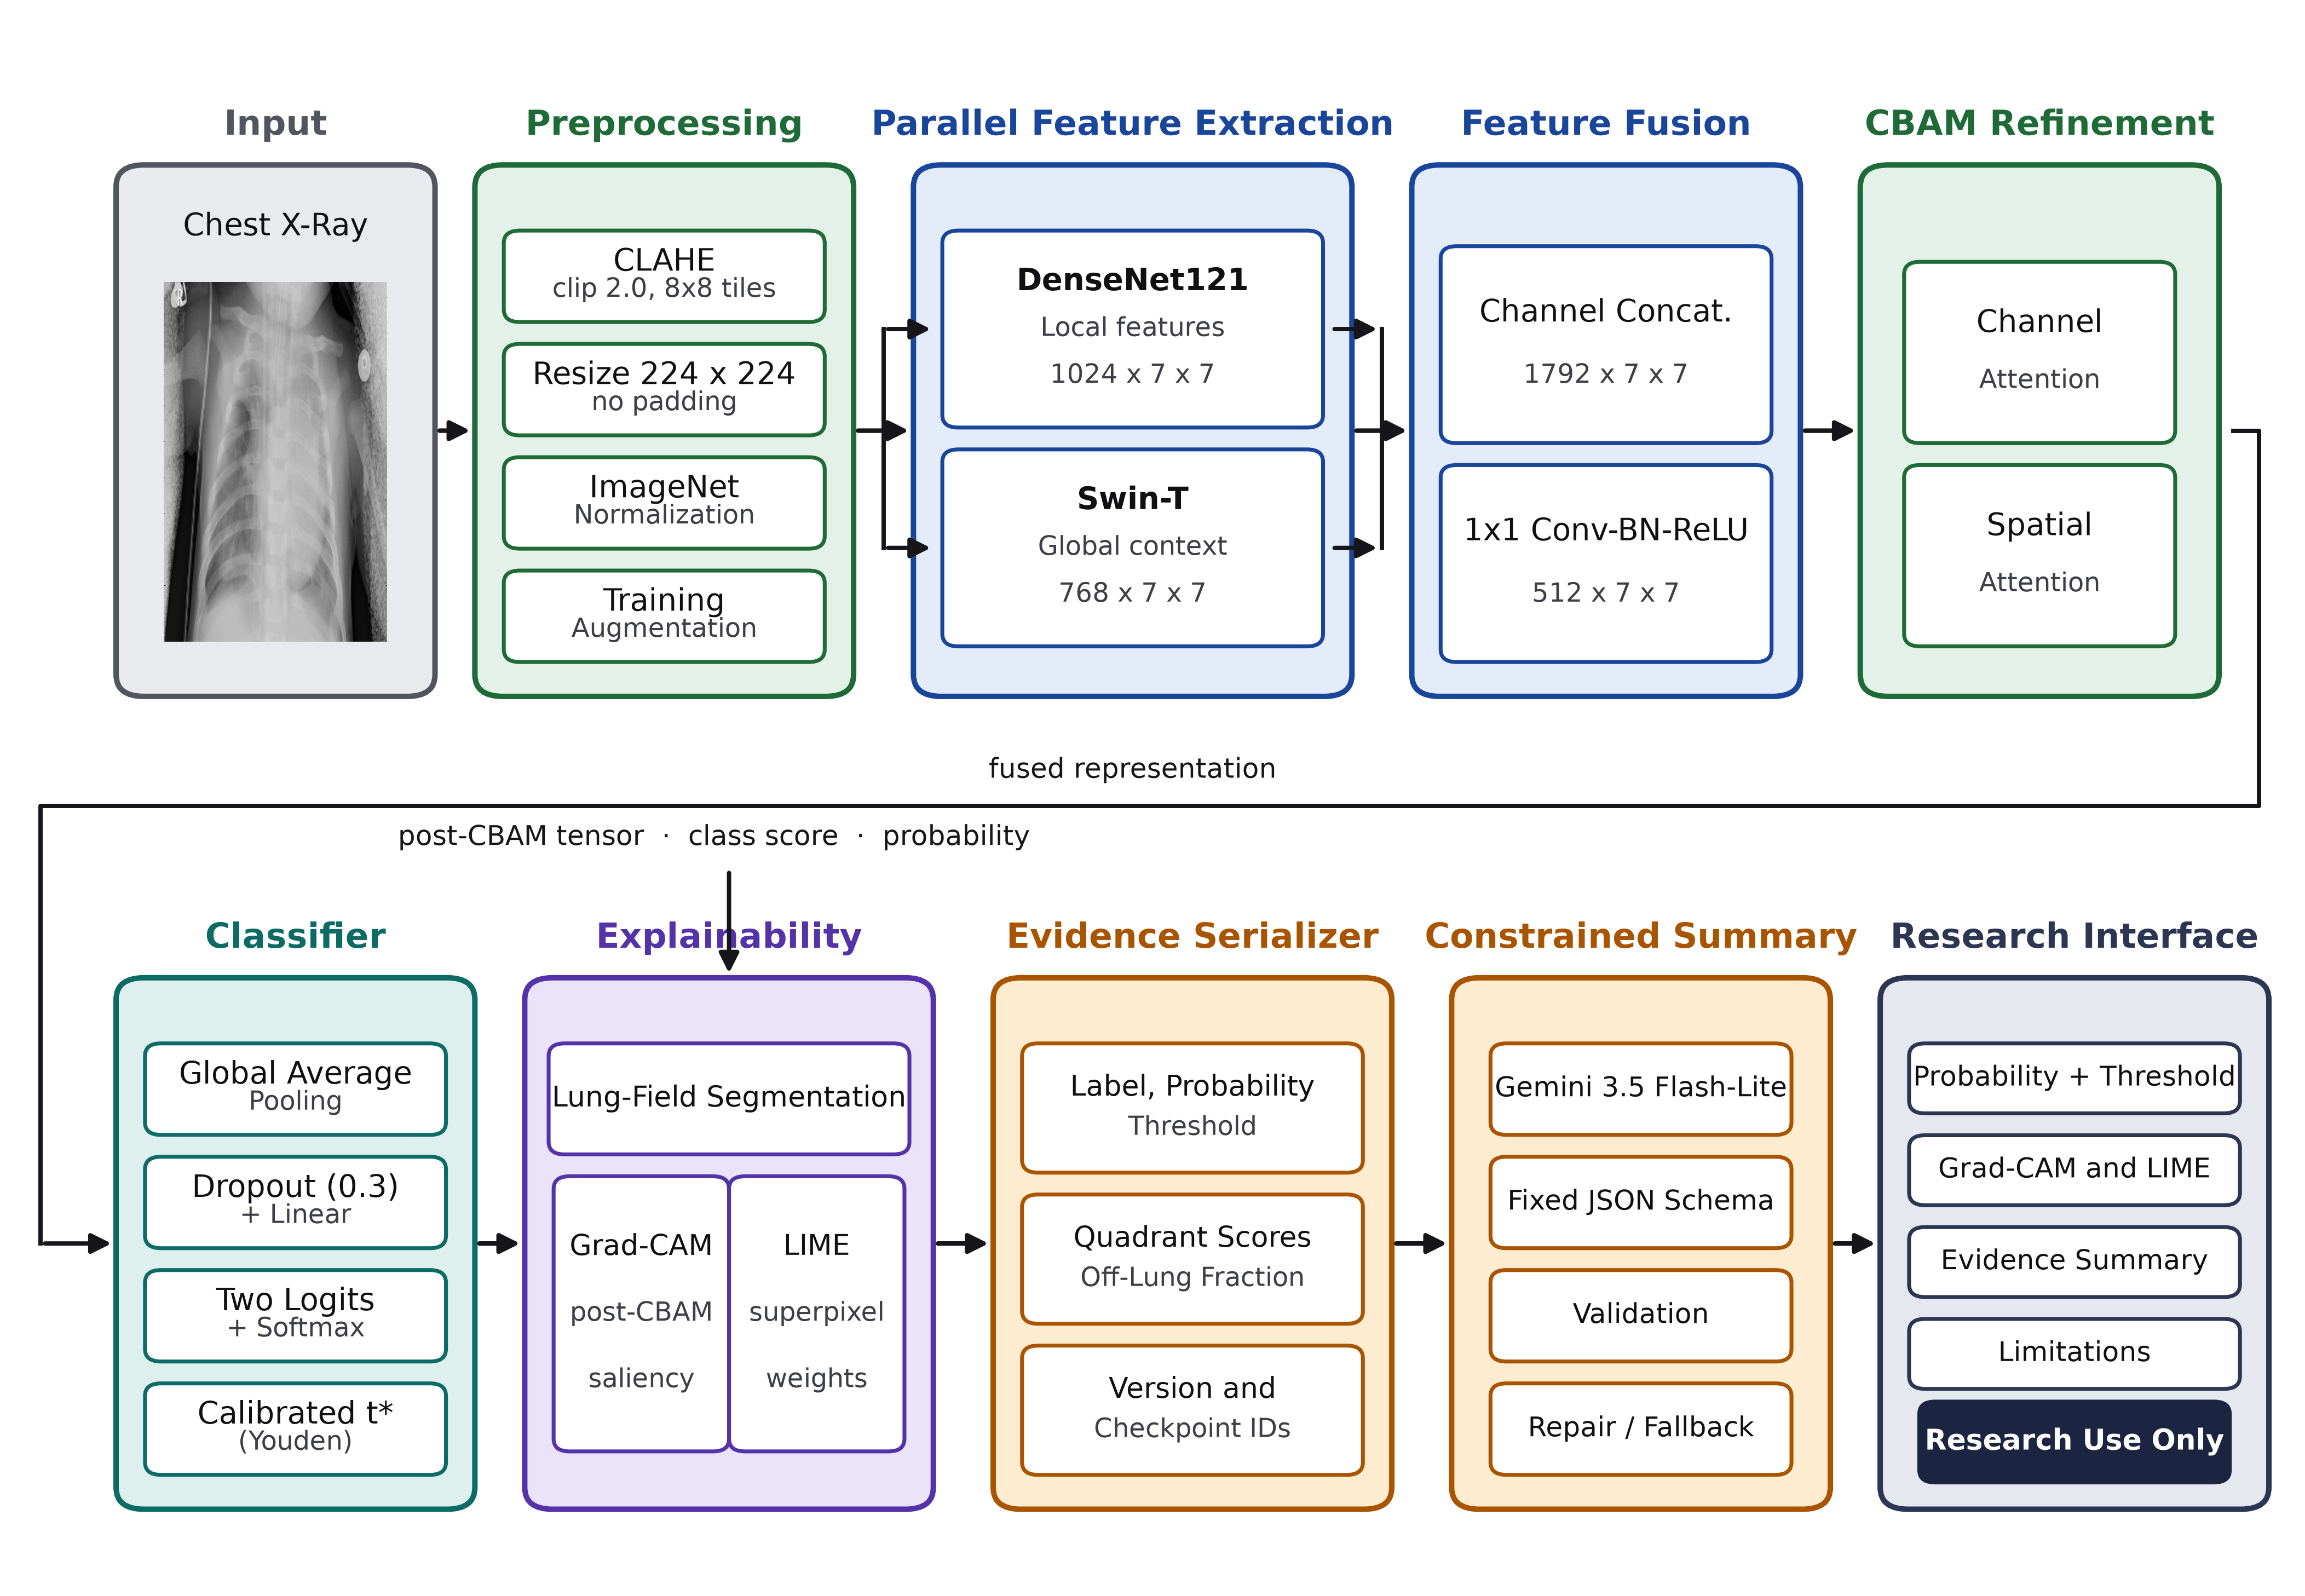
\includegraphics[width=0.92\textwidth]{architecture.png}
\caption{End-to-end classification, explanation, and evidence-constrained summarization workflow.}
\label{fig:architecture}
\end{figure*}

\subsection{Feature Extraction and Fusion}
DenseNet121 \cite{huang2017densenet} and Swin-T \cite{liu2021swin} are initialized with ImageNet weights and operate in parallel on the same preprocessed image. For a $224\times224$ input, the DenseNet121 trunk produces $\mathbf{F}_D\in\mathbb{R}^{1024\times7\times7}$. The final Swin-T stage produces a representation corresponding to $768$ channels on a $7\times7$ grid. An explicit adapter $\mathcal{A}$ converts the Swin output to channels-first (NCHW) layout before fusion.

The DenseNet and adapted Swin tensors are concatenated along the channel axis, giving a $1792\times7\times7$ tensor, which a $1\times1$ convolution--batch-normalization--ReLU block $\mathcal{P}_F$ projects to the 512-channel fused embedding used by CBAM and the classifier:
\begin{align}
\mathbf{F} &= \mathcal{P}_F\!\left([\mathbf{F}_D;\mathcal{A}(\mathbf{F}_S)]\right),
\qquad \mathbf{F}\in\mathbb{R}^{512\times7\times7}.
\label{eq:fusion}
\end{align}
Equation~\ref{eq:fusion} defines the project-specific fusion operation, where $[\cdot;\cdot]$ denotes channel concatenation. Runtime assertions check the layout and spatial dimensions before concatenation, helping to detect channels-last/channels-first mismatches. This explicit concatenation follows the general feature-level fusion pattern used in hybrid visual and multimodal systems \cite{swathi2021hybrid,swathi2023audiovisual}. Here, trainable projections place both radiographic feature tensors on a common spatial and channel basis.

\subsection{CBAM and Classification}
CBAM is applied once, after feature fusion, following the sequential channel- and spatial-attention formulation of Woo \emph{et al.} \cite{woo2018cbam}. Channel attention uses spatial average and maximum pooling followed by a shared multilayer perceptron. Spatial attention pools across channels and applies a $7\times7$ convolution:
\begin{align}
\mathbf{M}_c &= \sigma\!\left(\mathrm{MLP}(\mathrm{AvgPool}(\mathbf{F}))+
\mathrm{MLP}(\mathrm{MaxPool}(\mathbf{F}))\right), \nonumber\\
\mathbf{F}' &= \mathbf{M}_c\odot\mathbf{F}, \nonumber\\
\mathbf{M}_s &= \sigma\!\left(f^{7\times7}([\mathrm{AvgPool}_c(\mathbf{F}');
\mathrm{MaxPool}_c(\mathbf{F}')])\right), \nonumber\\
\mathbf{F}'' &= \mathbf{M}_s\odot\mathbf{F}'.
\label{eq:cbam}
\end{align}
In Eq.~\ref{eq:cbam}, $\sigma$ is the sigmoid function, $\odot$ is element-wise multiplication, and $[\cdot;\cdot]$ is channel concatenation. Pooling without a subscript runs over the spatial dimensions, so $\mathbf{M}_c\in\mathbb{R}^{C\times1\times1}$; the subscript $c$ marks pooling across channels, so $\mathbf{M}_s\in\mathbb{R}^{1\times H\times W}$. Both products in Eq.~\ref{eq:cbam} broadcast the attention map over the axes of size one. No residual path bypasses CBAM. Global average pooling, dropout with probability $0.3$, and a linear layer over the 512-channel embedding produce two logits, whose softmax gives $p$, the probability of pneumonia. The single-logit form below is equivalent for a two-class problem and states the class weighting more compactly:
\begin{align}
\mathbf{h}&=\mathrm{GAP}(\mathbf{F}''), \nonumber\\
\ell&=\mathbf{w}^{\top}\mathrm{Dropout}(\mathbf{h})+b,
\qquad p=\sigma(\ell), \nonumber\\
\mathcal{L}_{\mathrm{WBCE}}&=-\Big[\beta y\log p \nonumber\\
&\hspace{20mm}+(1-y)\log(1-p)\Big].
\label{eq:classifier}
\end{align}
The deployed configuration optimises the two-class focal form of Eq.~\ref{eq:classifier} with $\gamma=2$ and inverse-frequency class weights; the weighted binary cross-entropy below is the equivalent single-logit expression, retained because it states the class weighting compactly. In Eq.~\ref{eq:classifier}, $y=1$ denotes pneumonia and $y=0$ normal, and $\beta=N_0/N_1$ weights the positive term, with $N_0$ and $N_1$ the normal and pneumonia counts in the development set. Pneumonia is the majority class in this dataset, so $\beta\approx0.37$ rather than a value above one; the weight down-weights the abundant class, which is the same correction a value above one would apply had the minority class been positive. Training evaluates the equivalent logit-space expression through \texttt{BCEWithLogitsLoss}, which is numerically stable for large $|\ell|$. The operating threshold is selected from validation predictions using Youden's index \cite{youden1950index}:
\begin{align}
J(t)&=\operatorname{Sens}(t)+\operatorname{Spec}(t)-1,
\nonumber\\
t^*&=\arg\max_t J(t).
\label{eq:youden}
\end{align}
In Eq.~\ref{eq:youden}, $\operatorname{Sens}(t)$ and $\operatorname{Spec}(t)$ denote sensitivity and specificity at threshold $t$. The selected threshold $t^*$ is stored with the checkpoint; results at the fixed threshold $0.5$ are retained as a reference.

\subsection{Explainability and Evidence Serialization}
Grad-CAM \cite{selvaraju2017gradcam} targets the named post-CBAM tensor
$\mathbf{F}''$. For selected class score $s$, the channel weights and the
resulting low-resolution saliency map are
\begin{align}
\alpha_k&=\frac{1}{HW}\sum_{i,j}\frac{\partial s}{\partial F''_{kij}}, \nonumber\\
\widetilde{\mathbf{L}}_{\mathrm{GC}}&=\operatorname{ReLU}
\left(\sum_k\alpha_k\mathbf{F}''_k\right).
\label{eq:gradcam}
\end{align}
Equation~\ref{eq:gradcam} follows the original weighting. Here $H=W=7$ are the spatial dimensions of $\mathbf{F}''$ and $k$ indexes its
512 channels, so $\alpha_k$ is the spatially averaged gradient of $s$ with
respect to channel $k$. The head emits two logits, so the explanation targets
the logit of the predicted class directly. The displayed map is min--max
normalized to $[0,1]$. A named identity layer exposes the target tensor,
avoiding hooks that depend on library-specific internal names.

LIME \cite{ribeiro2016lime} uses SLIC superpixels \cite{achanta2012slic} and
fits a locally weighted sparse surrogate $g$ around image $\mathbf{x}$:
\begin{align}
\xi(\mathbf{x})&=\arg\min_{g\in\mathcal{G}}
\mathcal{L}(f,g,\pi_{\mathbf{x}})+\Omega(g), \nonumber\\
\mathcal{L}(f,g,\pi_{\mathbf{x}})
&=\sum_{(\mathbf{z},\mathbf{z}')\in\mathcal{Z}}
\pi_{\mathbf{x}}(\mathbf{z})
\big(f(\mathbf{z})-g(\mathbf{z}')\big)^2.
\label{eq:lime}
\end{align}
In Eq.~\ref{eq:lime}, $\mathbf{z}'$ marks which superpixels are retained,
$\mathbf{z}$ is the image that vector produces, $\mathcal{Z}$ is the sampled
set, $f(\mathbf{z})$ is the classifier probability, $\pi_{\mathbf{x}}$ weights
each sample by proximity to $\mathbf{x}$, and $\Omega(g)$ penalizes surrogate
complexity. The implementation requests 50 SLIC regions, evaluates 150
perturbations and retains the five highest-weighted regions at seed 42.

A deterministic serializer records the predicted label, probability,
threshold, Grad-CAM peak coordinates, heatmap concentration, LIME region
identifiers and signed weights, agreement indicators, preprocessing version
and checkpoint hash. It also reduces the saliency map to four radiographic
quadrants, reporting the dominant quadrant and a left/right balance ratio;
image left is the patient's right in the standard frontal convention. This
mapping is deterministic arithmetic over the map alone, with no segmentation
of anatomy and no detection of a lesion. Quadrant statistics cover the
segmented lung fields, not the full frame, so padding, chest wall and
sub-diaphragmatic structures do not dilute them. The segmentation comes from
a pretrained anatomical network distributed with TorchXRayVision
\cite{cohen2022torchxrayvision}, which labels left and right lung separately
from heart, mediastinum and diaphragm; only the two lung classes are kept.
Two simpler alternatives were discarded. An Otsu body mask retains shoulders,
clavicles and neck, and the contrast-limited equalization applied during
preprocessing removes the global intensity structure such a threshold needs.
A rule treating darker regions as lung fails in the opposite direction,
because consolidation is radiopaque: it excludes precisely the pathology an
explanation should show. The resulting zone label is the only spatial
language the summary may use, and the constraint enforced is not that spatial
terms are forbidden but that no field the serializer did not compute may
appear.

\subsection{Evidence-Constrained Summarization and Interface}
Gemini 3.5 Flash-Lite receives only the serialized evidence object and returns three JSON strings: \texttt{classification\_summary}, \texttt{model\_evidence}, and \texttt{limitations}. The request uses temperature $0$, a fixed prompt, and a fixed response schema. The application adds a non-generated research-use notice. Gemini models have been studied in medical tasks, but that evidence does not establish the correctness of this summarization pipeline \cite{saab2024gemini}.

The validator rejects missing or additional keys, non-string values, unsupported anatomy, diagnostic or treatment instructions, probability disagreements, and numbers absent from the evidence object. One bounded correction request reuses the same evidence and asks only for schema repair. If validation fails again or the service is unavailable, a deterministic template renders the same fields. The browser-based interface displays the input image, class probability and threshold, Grad-CAM overlay, LIME regions, serialized evidence, summary source, checkpoint version, and limitations.

\section{Implementation and Evaluation Setup}
\label{sec:setup}
\subsection{Training Configuration}
The model is implemented in PyTorch using \texttt{torchvision} and \texttt{timm}. Training uses AdamW \cite{loshchilov2019adamw} with cosine annealing, a batch size of 32, weight decay $10^{-4}$, and a maximum of 20 epochs. Training proceeds in two phases. The fusion, CBAM, and classification layers are first trained for eight epochs with both pretrained branches frozen, reading feature maps extracted once and cached. The complete network is then unfrozen and fine-tuned end to end for up to twelve epochs with discriminative learning rates, $10^{-4}$ for the new layers and $10^{-5}$ for the backbones, at a reduced batch size of 12 to fit the activations of both branches. Augmentation applies in the second phase only, since the cached features of the first are computed under deterministic preprocessing. Validation area under the receiver operating characteristic curve (AUROC) selects the checkpoint in both phases, with early stopping at a patience of five epochs. Results below are from single runs at seed 42; the prespecified seed set (42, 52, 62, 72, and 82) for repeated runs is not yet complete.

\begin{table}[t]
\centering
\caption{Controlled comparison configurations.}
\label{tab:baselines}
\scriptsize
\setlength{\tabcolsep}{3pt}
\begin{tabular}{L{2.2cm}L{4.4cm}}
\toprule
Configuration & Purpose \\
\midrule
DenseNet121 & CNN-only transfer-learning baseline \\
Swin-T & Transformer-only baseline \\
ResNet50 & Residual-CNN baseline \\
Fusion without CBAM & Isolates post-fusion attention \\
Complete classifier & DenseNet121--Swin-T fusion with CBAM \\
\bottomrule
\end{tabular}
\end{table}

\subsection{Comparison Protocol}
Every configuration in Table~\ref{tab:baselines} uses the same data partitions, deterministic preprocessing, augmentation policy, class-weighted loss, checkpoint rule, threshold procedure, seed set, and search budget. The ablation set also removes each feature branch separately. Explainability and language generation are applied after classification and do not alter the class probability.

\subsection{Metrics and Reproducibility}
Classification is scored with AUROC, area under the precision--recall curve,
sensitivity, specificity, precision, F1, balanced accuracy and the confusion
matrix. Calibration is reported separately, through the Brier score
\cite{brier1950verification}, expected calibration error
\cite{guo2017calibration} and reliability diagrams, since a classifier can
rank cases well and still be badly calibrated. Paired McNemar tests
\cite{mcnemar1947note} compare thresholded errors between configurations on
the same images; a paired bootstrap compares AUROC; a Holm correction
\cite{holm1979simple} covers the prespecified family. Both procedures
compare two classifiers on identical inputs, so they are informative from
single runs.

Explanation analysis covers deletion and insertion curves
\cite{petsiuk2018rise}, stability under small label-preserving
perturbations, map concentration and Grad-CAM/LIME agreement. No
localization score appears anywhere: the Kaggle release ships class labels,
not lesion masks, and scoring localization without them would report an
assumption as a measurement. Text analysis records schema-valid rate,
evidence agreement, forbidden-claim rate, fallback frequency,
reproducibility under identical inputs and latency, with the deterministic
template as the reference.

The displayed output is also reviewed by a practising clinician, credited in
the acknowledgment. Cases are drawn as a stratified sample before any result
is inspected, covering correct and incorrect predictions in both classes.
The reviewer sees the radiograph, the overlay and the generated summary, and
is blinded to which configuration produced them. Four items are scored on a
five-point scale: whether the highlighted region is plausible, whether the
summary is consistent with the displayed evidence, whether it avoids
unsupported clinical claims, and whether it is acceptable as a research-use
description. Each case is also marked for any statement that could be read
as a diagnosis. What this review establishes is narrow. It tests whether the
output is defensible to a reader with clinical training; it is not a
reference standard for the labels and does not replace the metrics above.

Reproducibility records include the dataset version, split manifest, file
hashes, source commit, environment lock file, library and CUDA versions,
hardware, seeds, checkpoint hashes, preprocessing parameters, threshold,
Grad-CAM target, LIME configuration, serializer and schema versions, prompt
hash, model identifier and API access date.

\section{Results}
\label{sec:results}
Results cover all five configurations of Table~\ref{tab:baselines} under the
protocol fixed in Section~\ref{sec:setup}. Every configuration was trained
once, at seed 42, and evaluated on the held-out 624-image test partition.
Single-run results cannot separate an architectural effect from seed
variation, and the margins reported below are small enough that this
limitation governs how they may be read; the point is made here so a reader need not infer it. Repeated runs across the prespecified seed
set remain outstanding, so no entry below carries a confidence interval
derived from them.

\subsection{Implementation Details}
Training was performed on a single NVIDIA T4. Inference and explanation figures in
this section were measured on an Apple M-series CPU under Python 3.14.0,
PyTorch 2.14.1, \texttt{torchvision} 0.29.1, and \texttt{timm} 1.0.30, with
the environment lock file recorded in Section~\ref{sec:setup}. The complete
classifier contains 35{,}425{,}632 trainable parameters, against 6{,}955{,}906
for DenseNet121 and 27{,}520{,}892 for Swin-T in isolation; removing CBAM
leaves 35{,}392{,}764, so the attention module accounts for 32{,}868
parameters, under $0.1\%$ of the total. The ResNet50 baseline contains 23{,}512{,}130 parameters. A single
run took 36 to 49 minutes depending on the configuration, roughly six minutes
of which is the one-off feature extraction that phase 1 caches; the five runs
reported here total about 3.5 GPU-hours. A full sweep over the prespecified
seed set would cost five times that.

\subsection{Classification Performance and Ablation}
Table~\ref{tab:main} carries the primary comparison and the ablation in one
block, since the single-branch rows serve both purposes and splitting them
would repeat the same six runs across two tables. Rows one and two isolate
each representation. Row three gives the residual CNN reference.
Row four keeps the fusion path but drops post-fusion CBAM, and row five is
the complete classifier. Two differences carry the architectural claims: rows
four against five for the attention module, and rows one and two against row
four for fusion itself.

Fusion separates from the single-branch baselines. Both fused
configurations exceed every baseline on accuracy, specificity, F1 and
balanced accuracy: $0.934$ and $0.920$ against $0.915$, $0.901$ and $0.897$.
The gain is concentrated in specificity, which rises from a $0.778$--$0.846$
band across the baselines to $0.914$ without CBAM and $0.855$ with it. Since
specificity is the weaker direction for every architecture tested, this is
where fusion contributes.

Post-fusion CBAM does not add to that. The configuration without it leads on
accuracy, AUROC, specificity, F1 and balanced accuracy, and the complete
classifier leads only on sensitivity ($0.959$). Section~\ref{sec:results}-D
tests whether that gap is real.

Every configuration remains more reliable at detecting pneumonia than at
recognising a normal radiograph, with sensitivity $0.933$--$0.959$ against
specificity $0.778$--$0.914$. This follows the class ratio of the
development set, in which pneumonia outnumbers normal by roughly $2.9{:}1$;
inverse-frequency weights of $1.939$ and $0.674$ were applied during
training, and the residual asymmetry is what those weights did not remove.
Confusion matrices at $t^*$ over the 624 test images are $214/20/21/369$
(TN/FP/FN/TP) for fusion without CBAM, $200/34/16/374$ for the complete
classifier, $198/36/17/373$ for DenseNet121, $182/52/10/380$ for Swin-T, and
$197/37/26/364$ for ResNet50.

\begin{table*}[t]
\centering
\caption{Test-set classification results at the validation-selected threshold $t^*$, on the held-out 624-image partition. All entries are single runs at seed 42 and carry no confidence interval; see Section~\ref{sec:discussion} on the size of the margins. Best value per column in bold. ECE is computed with 15 equal-width bins.}
\label{tab:main}
\scriptsize
\setlength{\tabcolsep}{4pt}
\begin{tabular}{L{2.9cm}C{1.9cm}C{1.9cm}C{1.9cm}C{1.9cm}C{1.9cm}C{1.6cm}C{1.3cm}}
\toprule
Configuration & AUROC & AUPRC & Sensitivity & Specificity & F1 & Bal.\ acc. & ECE \\
\midrule
DenseNet121         & 0.962 & 0.969 & 0.956 & 0.846 & 0.934 & 0.901 & \textbf{0.052} \\
Swin-T              & 0.975 & \textbf{0.983} & 0.974 & 0.778 & 0.925 & 0.876 & 0.054 \\
ResNet50            & 0.954 & 0.966 & 0.933 & 0.838 & 0.919 & 0.885 & 0.075 \\
Fusion without CBAM & \textbf{0.977} & 0.981 & 0.946 & \textbf{0.914} & \textbf{0.947} & \textbf{0.930} & 0.078 \\
Complete classifier & 0.974 & 0.972 & \textbf{0.959} & 0.855 & 0.937 & 0.907 & 0.062 \\
\bottomrule
\end{tabular}
\end{table*}

\subsection{Threshold Selection and Calibration}
For the DenseNet121 baseline the Youden threshold selected on validation was
$t^*=0.70$, well above the $0.5$ reference. That displacement is itself
informative: it is the magnitude by which the class imbalance pushes the
decision boundary, and applying the default $0.5$ instead costs specificity
on every borderline radiograph. The selected threshold is stored in the
checkpoint and applied unchanged at inference, so the deployed operating
point and the reported metrics describe the same classifier. Selected thresholds differ
substantially across configurations, from $0.422$ for Swin-T to $0.717$ for
fusion without CBAM, which is itself a reason to report each model at its
own operating point instead of a shared default.

Calibration is better than the spread of thresholded accuracies suggests.
Brier scores ranged from $0.062$ to $0.085$, with expected calibration
errors of $0.052$ to $0.078$ as listed in Table~\ref{tab:main}. Emitted
probabilities therefore track observed frequencies closely even where the
thresholded decisions diverge, supporting the reading that these
configurations differ more in where they cut than in how they rank.
Fig.~\ref{fig:roc} gives the reliability curves over 15 equal-width bins.

\begin{figure}[t]
\centering
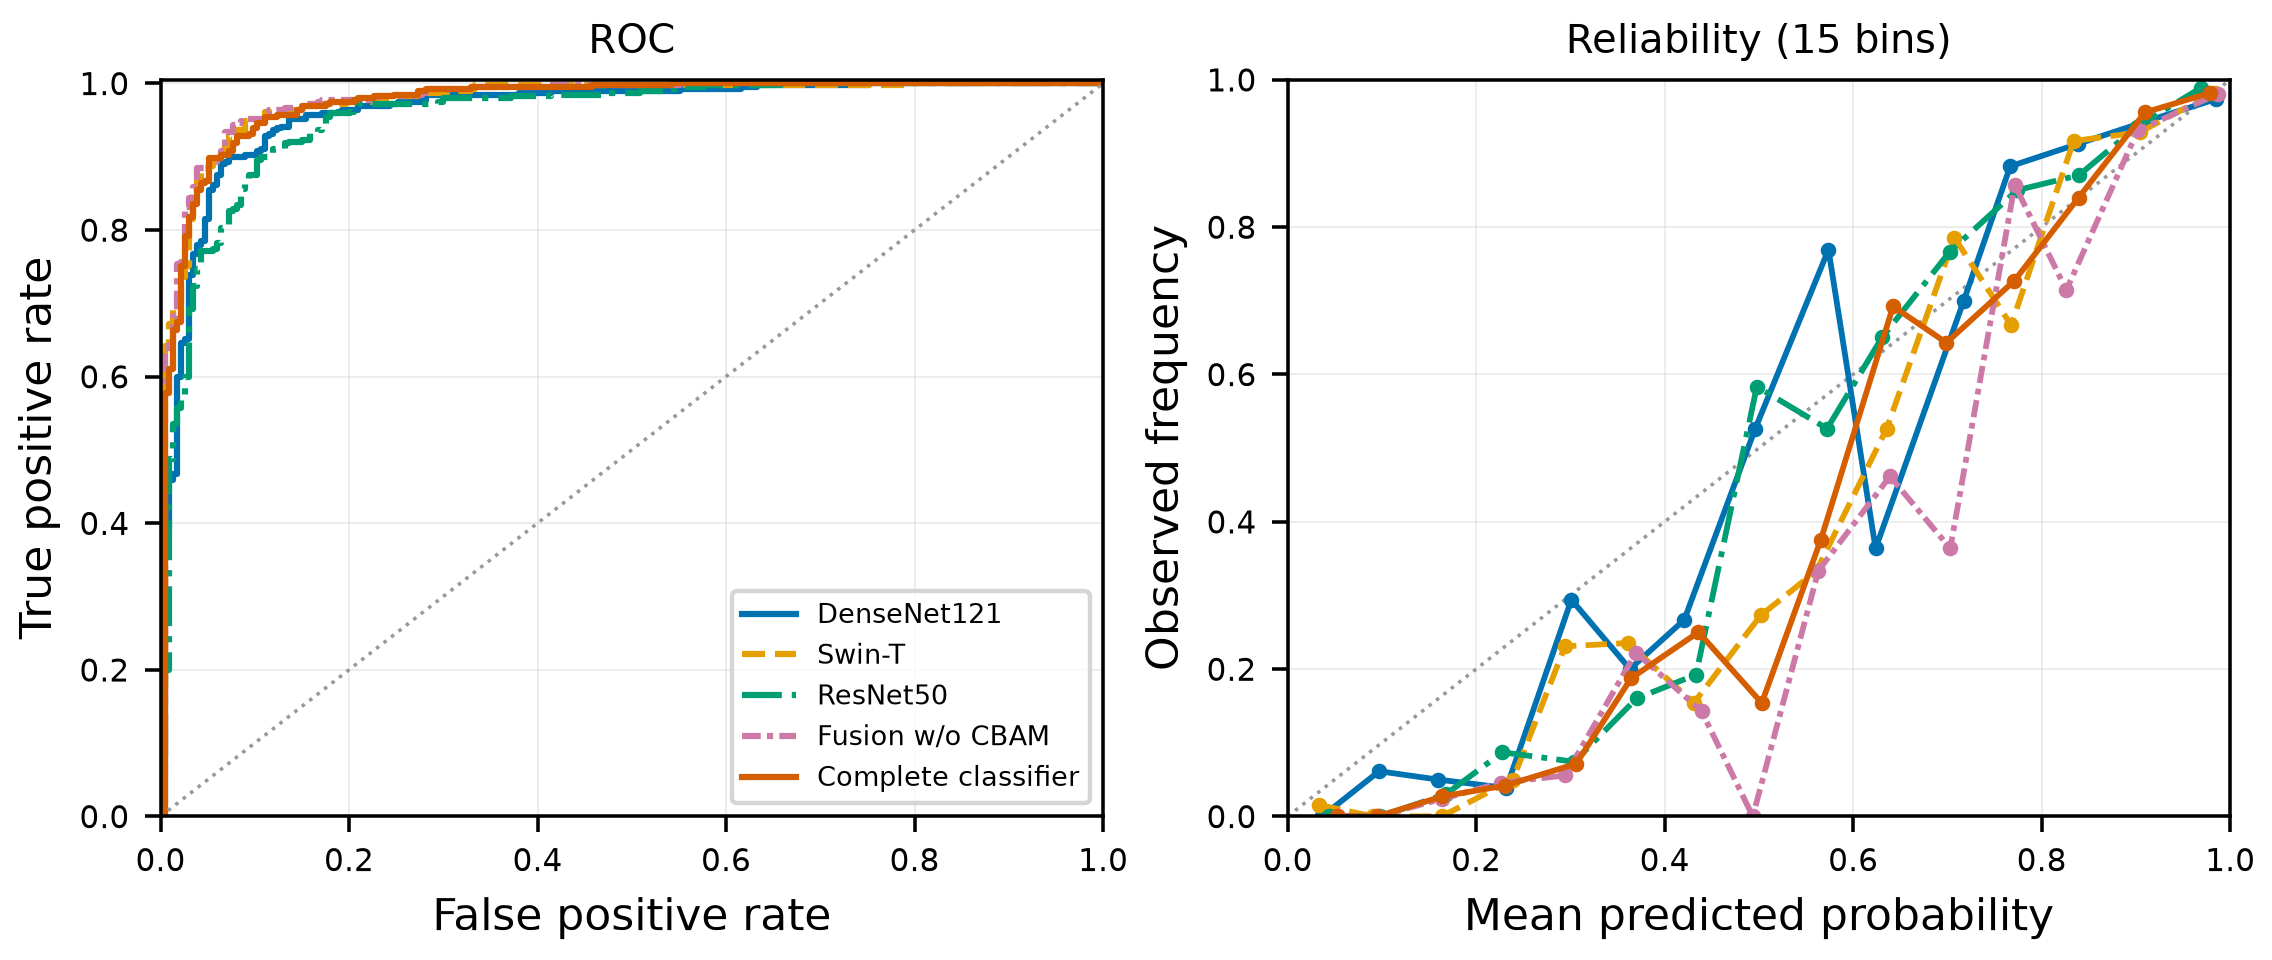
\includegraphics[width=\columnwidth]{fig_roc_reliability.png}
\caption{Discrimination and calibration on the held-out test partition. ROC curves for all five configurations (left) and reliability curves over 15 equal-width bins (right).}
\label{fig:roc}
\end{figure}

\subsection{Statistical Comparison}
Table~\ref{tab:stats} reports the paired comparisons, with $p$-values
Holm-adjusted across the four.

The ablation does not support the attention module. Against fusion without
CBAM, the complete classifier is correct on 9 radiographs its ablated
counterpart misses and incorrect on 18 that the ablated model gets right,
giving $p=0.244$; the AUROC difference is $-0.003$ with an interval spanning
zero. Post-fusion CBAM therefore produces no measurable improvement here.
The point estimates favour the ablated configuration, but not
significantly, so the defensible claim is an absence of effect, not a
reversal.

No comparison against the single-branch baselines reaches significance after
correction either. The closest is Swin-T, discordant 20 against 8 with an
unadjusted $p=0.036$ that becomes $0.143$ once the family is accounted for;
against DenseNet121 the complete classifier is effectively tied, 18 against
15. Accuracy differences of one to two points on 624 images are not
resolvable from a single run, and that column should not be read as a
ranking.

Discrimination behaves differently. The complete classifier attains a
significantly higher AUROC than DenseNet121 ($+0.012$) and ResNet50
($+0.019$), with bootstrap intervals excluding zero in both cases, while
being indistinguishable from Swin-T and from its own ablation. Fusion
improves ranking over the convolutional baselines even where the thresholded
decisions are statistically tied.

\begin{table}[t]
\centering
\caption{The complete classifier against each other configuration, on the same 624 test images. McNemar compares thresholded errors; $\Delta$AUROC uses a paired bootstrap with 2{,}000 resamples. $p$-values are Holm-adjusted across the four comparisons.}
\label{tab:stats}
\scriptsize
\setlength{\tabcolsep}{3.5pt}
\begin{tabular}{L{2.4cm}C{2.2cm}C{1.0cm}C{1.0cm}}
\toprule
Comparison & $\Delta$AUROC [95\% CI] & McN.\ $p$ & Holm $p$ \\
\midrule
vs.\ DenseNet121         & $+0.012$ [$+0.005$, $+0.020$] & 0.728 & 0.728 \\
vs.\ Swin-T              & $-0.001$ [$-0.006$, $+0.003$] & 0.036 & 0.143 \\
vs.\ ResNet50            & $+0.019$ [$+0.009$, $+0.031$] & 0.065 & 0.195 \\
vs.\ Fusion without CBAM & $-0.003$ [$-0.006$, $+0.001$] & 0.122 & 0.244 \\
\bottomrule
\end{tabular}
\end{table}

\subsection{Explanation Behavior}
Table~\ref{tab:xai} summarizes explanation behavior for the complete
classifier. Deletion and insertion scores \cite{petsiuk2018rise} ask whether
removing or restoring the highest-ranked regions moves the class probability
the way the explanation implies it should. Stability is the mean rank
correlation between an image's explanation and that of a three-pixel
translation, realigned before comparison. Agreement is the
intersection-over-union of the top-quintile regions of the two maps. None of
these is a localization score: the dataset carries no lesion annotations, so
every entry describes model sensitivity and nothing about anatomical
correctness.

LIME is the more faithful of the two, with a lower deletion AUC ($0.581$
against $0.616$), a higher insertion AUC ($0.789$ against $0.724$) and more
concentrated maps. It costs some 45 times as much, $8.17$ s per image
against $0.18$ s, so Grad-CAM is the default view and LIME is computed on
request. Grad-CAM is stable under small translations ($\rho=0.81$).

The two agree only weakly, at an IoU of $0.203$: two attribution methods
applied to the same model and image select largely different regions, so
neither can be treated as the account of what the model used. That is partly
expected from their assumptions, since Grad-CAM weights a $7\times7$ tensor
by gradients and is coarse, while LIME occludes SLIC superpixels and returns
a sparse selection. Convergence is evidence and divergence is a warning,
and both are displayed for that reason.

\begin{table}[t]
\centering
\caption{Explanation and summarization behavior for the complete classifier. Grad-CAM over 25 test radiographs, LIME over 8 at 150 perturbations, summaries over 20. Agreement is the IoU of the top-quintile regions of the two maps. The deterministic template is correct by construction on the schema, evidence and repeat rows and is the reference, not a competing method.}
\label{tab:xai}
\scriptsize
\setlength{\tabcolsep}{4pt}
\begin{tabular}{L{3.5cm}C{1.5cm}C{1.5cm}}
\toprule
\multicolumn{3}{l}{\textit{(a) Explanation}} \\
Measure & Grad-CAM & LIME \\
\midrule
Deletion AUC (lower better)   & 0.616 & \textbf{0.581} \\
Insertion AUC (higher better) & 0.724 & \textbf{0.789} \\
Map concentration             & 0.288 & 0.387 \\
Stability under perturbation  & 0.810 & --- \\
Mean runtime per image (s)    & \textbf{0.18} & 8.17 \\
Grad-CAM / LIME agreement (IoU) & \multicolumn{2}{c}{0.203} \\
\midrule
\multicolumn{3}{l}{\textit{(b) Summarization}} \\
Measure & Gemini & Template \\
\midrule
Schema-valid (\%)            & 100 & 100 \\
Evidence agreement (\%)      & 85 & 100 \\
Forbidden claim (\%)         & 0 & 0 \\
Fallback invoked (\%)        & 0 & --- \\
Bit-identical on repeat (\%) & 0 & 100 \\
Mean latency (s)             & 7.9 & 0.02 \\
\bottomrule
\end{tabular}
\end{table}

Three implementation findings bear on how these maps should be read, each
settled by measurement rather than by eye against an occlusion-sensitivity
reference: each $32\times32$ patch of the input is blanked in turn and the
drop in predicted probability recorded.

The target tensor is not a neutral choice. For DenseNet121, attaching
Grad-CAM to the final $1024$-channel block output instead of to the last
convolution inside the terminal dense layer, which emits only the $32$ new
growth-rate channels, lowered the deletion AUC from $0.723$ to $0.683$. For
ResNet50, targeting the whole terminal block instead of its last convolution
raised agreement from $r=0.23$ to $r=0.31$, because the convolution's output
has yet to pass through the residual addition the pooled feature depends on.
For the complete classifier, hooking the spatial-attention convolution
inside CBAM captures a single-channel attention mask, not the refined
feature tensor; only two of six sample peaks then fell inside the lung
fields, against six of six once the module output was targeted.

A layout mismatch can invert an attribution outright. The Swin branch emits
channels-last activations and the attribution library assumes
channels-first; read in the wrong layout the maps correlated $r=-0.12$ with
the occlusion reference, highlighting regions the model demonstrably did not
use. An explicit layout adapter moved the same configuration to $r=+0.31$. A
negative correlation is the only reliable signal that such a bug exists,
since the maps stay visually plausible throughout.

With all corrected, agreement is positive everywhere but markedly weaker for
the fused models: $r=0.27$ to $0.31$ for the single-branch baselines against
$r=0.10$ for the complete classifier and $r=0.04$ for its ablation.
Attribution through a fused representation is harder, since the gradient at
the fusion point mixes two backbones with different inductive biases and one
map must summarise both. The fused models classify better and explain less
faithfully, a trade-off worth stating in a system whose purpose is to show
its reasoning.

Before masking, between $21\%$ and $48\%$ of saliency mass fell outside the
segmented lung fields, and on normal radiographs the global maximum often
lay over the clavicles or the image border. Explanations are therefore
confined to lung fields for display and for the zone statistics, with the
off-lung fraction carried alongside.

\begin{figure}[t]
\centering
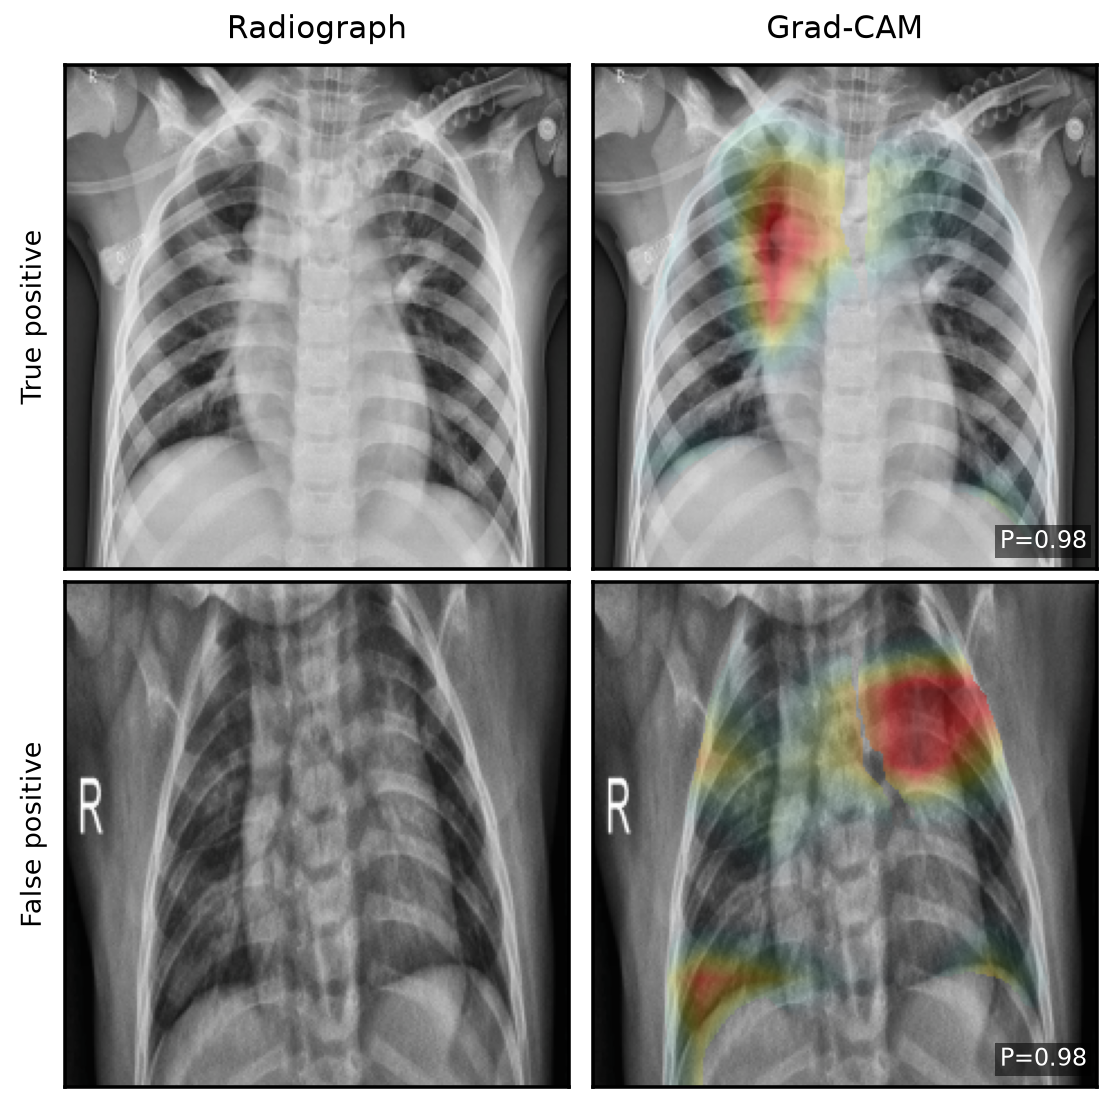
\includegraphics[width=0.70\columnwidth]{fig_qualitative.png}
\caption{Qualitative output of the complete classifier on four held-out cases, including one false positive and one false negative. $P$ is the predicted probability of pneumonia. Highlighted regions indicate model sensitivity confined to the segmented lung fields; they are not radiological findings.}
\label{fig:qualitative}
\end{figure}

Fig.~\ref{fig:qualitative} shows correct and incorrect cases under identical
display settings. The misclassified rows matter more: explanation maps stay
confident when the prediction is wrong, and making that visible is why the
probability, the threshold and the evidence object accompany every overlay.

\subsection{Evidence-Constrained Summarization}
Table~\ref{tab:xai}(b) sets the constrained Gemini summaries against the
deterministic template on identical evidence objects. The forbidden-claim
rate counts summaries containing anatomical localization beyond the computed
quadrants, diagnostic language or treatment instruction. The final row
records whether repeated requests with identical evidence, a fixed prompt and
temperature $0$ return byte-identical text.

Schema compliance was complete: all 20 summaries carried every required
section, no repair request was needed and the fallback was never invoked. No
summary contained lobar anatomy the serializer does not compute or any
treatment instruction. Evidence agreement was $85\%$; three of twenty
described the classifier's confidence qualitatively without restating the
figure, which the validator counts as a disagreement because it cannot
verify an absent number.

Repeatability was zero. Temperature $0$ did not produce byte-identical text
on any repeat, which matters here more than it would elsewhere: if the same
evidence can yield differently worded summaries, the text is not a
deterministic function of the model's output, and an audit trail must store
the generated summary instead of regenerating it. The system does store it.

One template change is worth recording, because reading the output prompted
it, not a metric. The initial template asserted focal airspace consolidation
in the dominant saliency zone and recommended initiating empiric
antimicrobial therapy, in identical wording at $71\%$ and at $99\%$
confidence. Both exceed what a probability and a saliency peak support.
Certainty language is now tiered by confidence, the findings sentence
attributes the location to the model's region of maximal response instead of
to observed consolidation, and the treatment directive has been removed.

\subsection{Clinical Review}
\label{sec:review}
A practising clinician with \TBD{} years of reporting experience, named in
the acknowledgment, reviewed \TBD{} stratified test cases under the blinded
protocol of Section~\ref{sec:setup}. Table~\ref{tab:expert} gives the mean
score for each rubric item and the share of cases flagged as carrying a
statement that could be read as a diagnosis. The reviewer judged
presentation, not labels. Review notes recorded \TBD{} as the most frequent
objection, and \TBD{} cases came back with a request to reword the
summary.

\begin{table}[t]
\centering
\caption{Blinded clinical review of \TBD{} stratified test cases. Scores are means on a five-point scale. The reviewer is credited in the acknowledgment.}
\label{tab:expert}
\scriptsize
\setlength{\tabcolsep}{4pt}
\begin{tabular}{L{4.4cm}C{1.3cm}C{1.3cm}}
\toprule
Rubric item & Correct & Incorrect \\
 & cases & cases \\
\midrule
Plausibility of highlighted region  & \TBD & \TBD \\
Consistency with displayed evidence & \TBD & \TBD \\
Absence of unsupported claims       & \TBD & \TBD \\
Overall acceptability, research use & \TBD & \TBD \\
\midrule
Cases flagged as diagnosis-like (\%) & \TBD & \TBD \\
\bottomrule
\end{tabular}
\end{table}

\subsection{Latency}
Latency was measured on an Apple M-series CPU with no GPU acceleration.
Preprocessing costs $16$ ms, the forward pass $21$--$31$ ms, Grad-CAM under
$100$ ms, and template rendering with PDF generation a further $16$ ms.
Lung-field segmentation adds roughly $950$ ms and is by a wide margin the
largest local cost, the price of replacing the intensity heuristics of
Section~\ref{sec:method}; it runs once per image, independent of the
classifier. End-to-end latency is near $1.1$ s with the deterministic
template and $5$--$6$ s with the live service, which then dominates. LIME is
excluded at $8.2$ s per image, some 45 times Grad-CAM, so it is computed on
request. The pipeline is interactive on commodity hardware without a GPU,
the constraint a teaching deployment imposes.

\section{Discussion}
\label{sec:discussion}
The ablation does not support one of this paper's own design choices. Against
the otherwise identical configuration without it, the complete classifier
wins 9 radiographs and loses 18, at a Holm-adjusted $p=0.244$, with an AUROC
difference whose interval spans zero. The same direction appeared under an
earlier frozen-backbone protocol, so it is not an artefact of one training
regime. Only one reading is supported: CBAM is not shown to degrade
performance, because the gap is not significant, and it is not shown to help
either. For $32{,}868$ parameters the module earns no place here.

Fusion itself fares better. Both fused configurations exceed every
single-branch baseline on accuracy, specificity, F1 and balanced accuracy,
and the complete classifier attains significantly higher AUROC than
DenseNet121 and ResNet50. The gain concentrates in specificity, the weak
direction for every architecture tested. Combining a convolutional and a
transformer branch is justified by this evidence; refining the fused tensor
with attention is not.

Beyond that, the accuracy column is not a ranking. No comparison in
Table~\ref{tab:stats} survives correction, and a one- to two-point gap on
624 images is not resolvable from a single run. What does separate the
configurations is the operating point. Swin-T achieves the best AUROC,
$0.975$, and the worst specificity, $0.778$: it ranks radiographs well and
then commits to pneumonia too readily, returning 52 false positives against
the complete classifier's 30. Ranking quality and decision quality come
apart, so the contribution of fusion is a balanced decision boundary, not
superior discrimination.

One asymmetry runs through every row. All five configurations detect
pneumonia more reliably than they recognise a normal radiograph, at
sensitivity $0.933$--$0.974$ against specificity $0.778$--$0.914$.
Inverse-frequency weights were applied throughout and did not remove it: the
$2.9{:}1$ class ratio of the development set survives into the decision
behaviour of every architecture. Any deployment reading should begin there,
because the error the system makes most often is calling a healthy chest
abnormal.

The explanation results are weaker than the classification results and
should be read as such. Grad-CAM and LIME agree at an IoU of $0.203$, which
is low for two methods applied to the same model and image; agreement with
an occlusion reference is modest for the baselines and weak for the fused
models. Convergence between the two is therefore evidence and divergence is
a warning, and neither is a finding about consolidation. No localization
score appears anywhere in this paper for a related reason: computing one
would need lesion annotations the dataset does not contain, and a number
produced without them would report an assumption as a measurement.

Separating the classifier from the language model is what makes
Table~\ref{tab:xai} interpretable. The model never sees the radiograph and
never receives an anatomical label, so a factual error in a summary must
originate either in the serialized evidence or in a schema violation, and
both are machine-checkable. The deterministic template is correct by
construction on those rows, which bounds what constrained generation can add
to readability alone. That the generated text is not reproducible across
repeats is the reason the system stores each summary instead of
regenerating it.

One deployment failure is worth recording because it is invisible to the
usual checks. The evaluation script read the calibrated threshold from the
checkpoint while the serving path applied \texttt{argmax}, so the deployed
decision boundary silently reverted to $0.5$ while the reported sensitivity
and specificity continued to describe $t^{*}$. The test suite passed
throughout, because it verified output shapes and response codes, never
agreement between the two paths. A threshold selected and reported but not
applied is indistinguishable, from the outside, from one that was never
selected; regression tests now assert that the served threshold equals the
stored one.

Several results depend on choices that could have gone the other way. CBAM
is applied once after fusion, which keeps the Grad-CAM target unambiguous
but leaves branch-specific features unrefined. Fusion is concatenation with
a learned projection, not cross-attention: cheaper and easier to assert
shape invariants over, and unable to let either branch condition on the
other. Youden's index weights sensitivity and specificity equally, which is
not the operating point a screening deployment would choose. Each is
recorded so the numbers are read against the configuration that produced
them.

\section{Limitations, Ethics, and Privacy}
\label{sec:limits}
The Kaggle dataset holds pediatric images from one institution and is
strongly class-imbalanced. Its public directory structure carries no
dependable patient identifier, so an image-level partition cannot establish
patient-level independence. The binary labels collapse bacterial and viral
pneumonia into a single class. Every configuration was trained once, so no
result here separates an architectural effect from seed variation, and the
paired tests report only that differences are not resolvable at this sample
size. Nothing extends to other ages, institutions, devices or acquisition
protocols without external validation.

Measured saliency on the trained models falls substantially outside the
thorax, between $21\%$ and $48\%$ of total mass, and on normal radiographs
the global maximum often lay outside the lung fields. Because an occlusion
reference agrees with these maps, the behaviour is attributable to the
classifier, not to the attribution method, and it is consistent with the
shortcut learning this dataset is known to permit: systematic differences in
framing, cropping and acquisition between the two class folders are
predictive without reference to lung parenchyma. Masking the explanation to
segmented lung fields improves what is displayed but does not alter what the
model uses. Lung-field cropping during preprocessing is the appropriate
mitigation and is not yet applied.

Grad-CAM and LIME visualize model sensitivity, not pathology and not causal
reasoning. Their outputs can be unstable, they agree only weakly with each
other, and an image coordinate is not an anatomical finding. Schema
validation enforces form and evidence consistency; it cannot enforce medical
correctness. The clinical review rests on one reader and a stratified
sample, so it supports statements about how the output is presented, not an
inter-reader agreement estimate, and it is not a clinical validation.

The dataset contains de-identified images handled under its source terms. No
patient identifier or source image is sent to the language service; only the
serialized evidence object is transmitted. Logs exclude sensitive metadata,
access is controlled, and the interface identifies whether text came from the
language service or the deterministic fallback. The system is restricted to
technical research and education and does not provide diagnosis, treatment,
triage or autonomous decision support.

\section{Conclusion}
The pipeline joins DenseNet121 and Swin-T representations through explicit projection and fusion, applies CBAM once to the fused tensor, and emits a binary pneumonia probability. Grad-CAM and LIME expose complementary aspects of model behavior. Deterministic serialization keeps the language model away from the source image, and schema validation with a template fallback leaves every displayed sentence traceable to a recorded field. What the workflow connects is classification, explanation, and readable output. What it deliberately does not do is convert model sensitivity into a medical claim.

\section*{Acknowledgment}
The authors thank \TBD{} (\TBD{}, \TBD{}) for the blinded review of the
explanation overlays and generated summaries reported in
Section~\ref{sec:review}, and for the comments recorded there. The review
was carried out without sight of the configuration labels, and the reviewer
received no compensation. Responsibility for the system, the analysis, and
any error in this paper rests with the authors.

\bibliographystyle{IEEEtran}
\bibliography{references}

\end{document}
